\mcchap{Le dashboard}{cap:dashboard}
In questo capitolo, a titolo di esempio verranno presentate delle immagini relative alle schermate estratte dall'applicazione.
È possibile visualizzare l’andamento dei contagi riferito 1, 3, 6 mesi e per tutto il periodo a partire da marzo 2020.
Tutti i grafici contenuti nella dashboard, sono interattivi.
Passando con il cursore del mouse sopra al grafico, vengono evidenziate le barre che indicano il numero dei contagi per quel determinato giorno.
Sul grafico è possibile agire sull'intervallo di tempo selezionando uno dei pulsanti indicati nel riquadro 1 della figura, oppure cliccando sulla legenda del riquadro 2, cambiare la configurazione delle tracce.
\begin{figure}[htp]
    \centering
    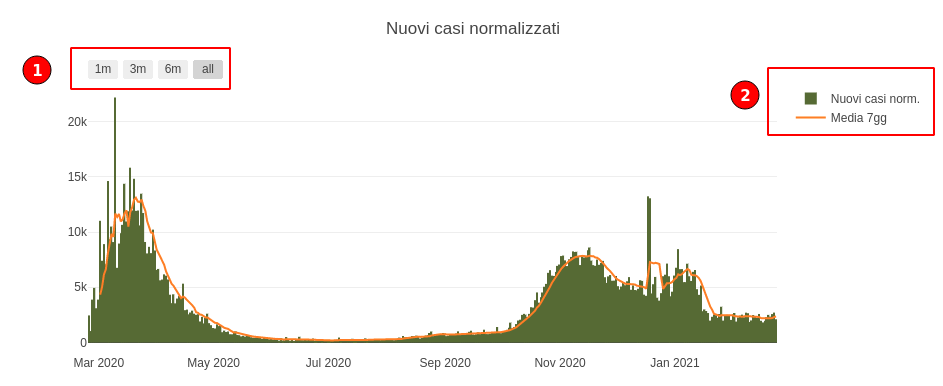
\includegraphics[width=14cm]{chart_explained}
    \caption{Esempio grafico}
\end{figure}
\section{Dashboard Italia}
Nella dashboard Italia sono presenti nove diversi grafici che illustrano l’andamento della pandemia attraverso le curve di contagi, le ospedalizzazioni, le terapie intensive e i decessi.
\subsection{Nuovi casi}
La figura \ref{fig:nuovi_casi} mostra il numero di nuovi casi giornalieri in Italia a partire dall'inizio della pandemia.
In ascissa sono riportati i giorni, e in ordinata il numero dei nuovi casi riportati in quel determinato giorno.
\begin{figure}[htp]
    \centering
    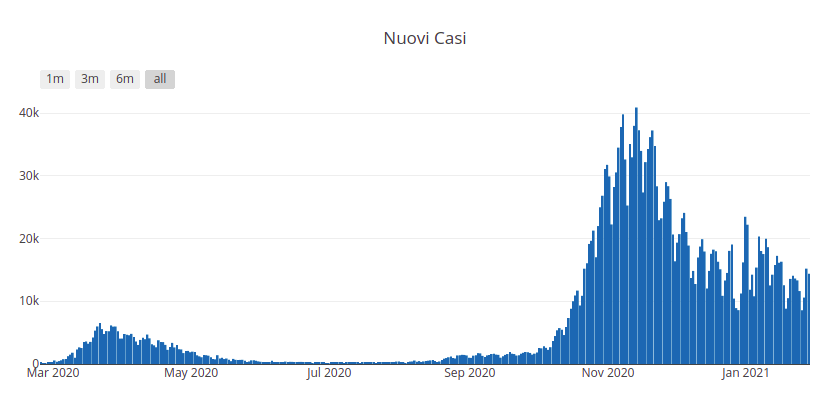
\includegraphics[width=14cm]{nuovi_casi}
    \caption{Nuovi casi}
    \label{fig:nuovi_casi}
\end{figure}

\subsection{Totale casi}
Nella figura \ref{fig:totale_casi} sono rappresentati i casi totali delle persone che hanno contratto il virus, che comprende gli attuali positivi, i guariti e i decessi.
\begin{figure}[htp]
    \centering
    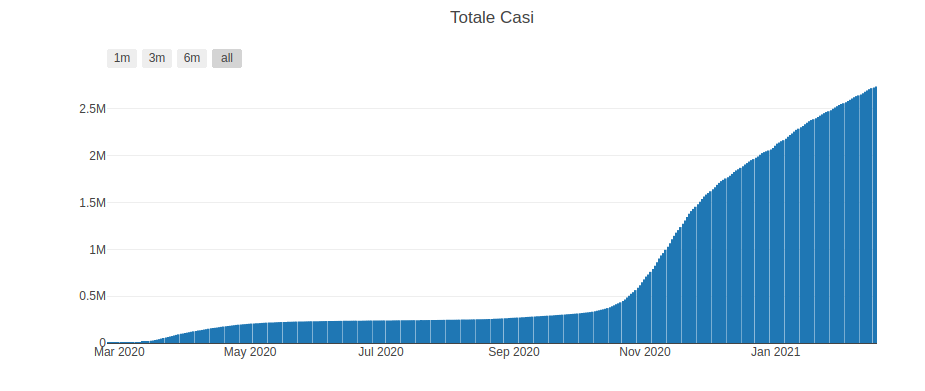
\includegraphics[width=14cm]{totale_casi}
    \caption{Totale casi}
    \label{fig:totale_casi}
\end{figure}

\subsection{Isolamento domiciliare}
Nella figura \ref{fig:isolamento_domiciliare} è raffigurato il grafico delle persone che si trovano in isolamento presso il loro domicilio.
\begin{figure}[htp]
    \centering
    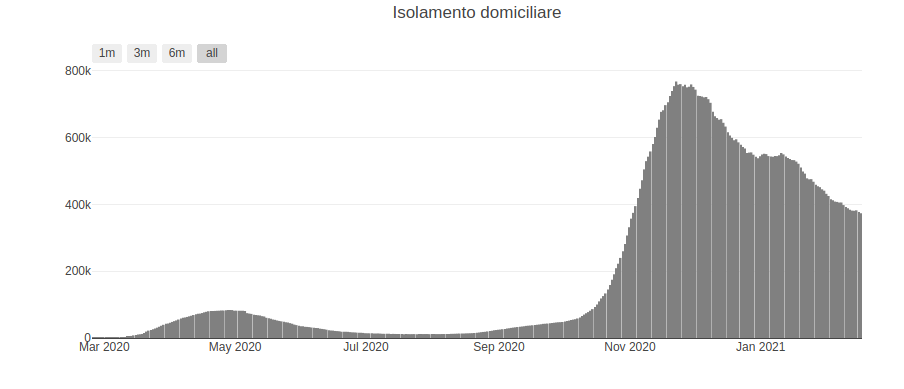
\includegraphics[width=14cm]{isolamento_domiciliare}
    \caption{Isolamento domiciliare}
    \label{fig:isolamento_domiciliare}
\end{figure}

\subsection{Terapia intensiva}
La figura \ref{fig:terapia_intensiva} mostra l'andamento dei pazienti ricoverati in ospedale in terapia intensiva dall'inizio della pandemia.
In blu si può osservare la linea che indica la media mobile a 7 giorni.
\begin{figure}[htp]
    \centering
    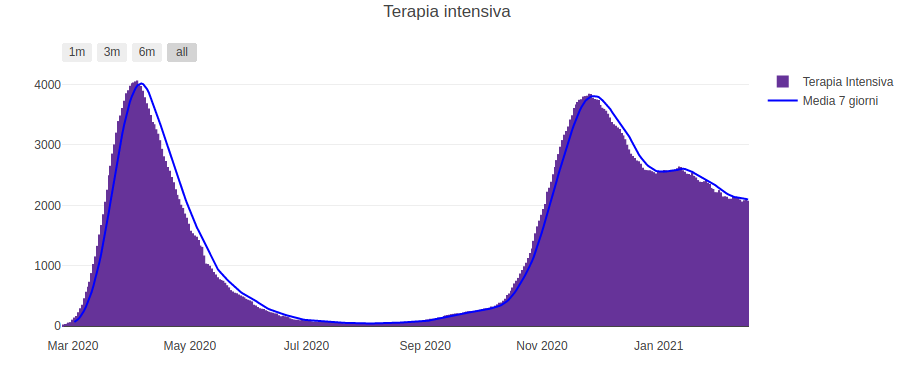
\includegraphics[width=14cm]{terapia_intensiva}
    \caption{Terapia intensiva}
    \label{fig:terapia_intensiva}
\end{figure}

\subsection{Casi normalizzati}
Il grafico nella figura \ref{fig:casi_normalizzati} mostra il numero di casi normalizzati, ossia resi indipendente dai tamponi effettuati ogni giorno.
In arancione è indicata anche la linea della media mobile a 7 giorni.
\begin{figure}[htp]
    \centering
    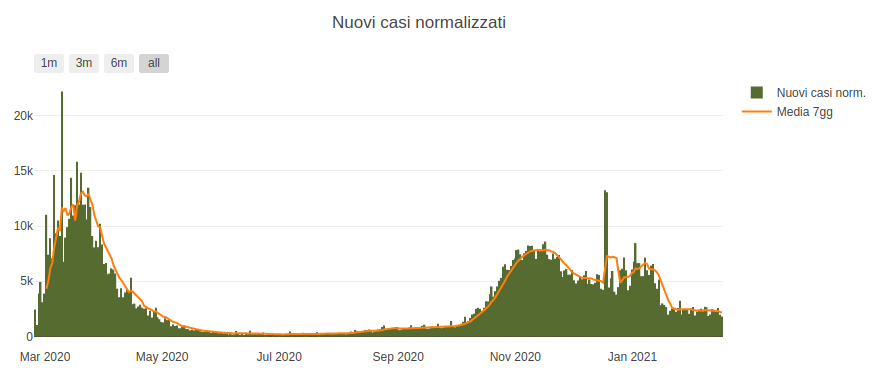
\includegraphics[width=14cm]{casi_norm}
    \caption{Casi normalizzati}
    \label{fig:casi_normalizzati}
\end{figure}

\subsection{Terapia intensiva e ospedalizzati}
Nel grafico della figura \ref{fig:ti_ospdedalizzati} è possibile osservare l'andamento delle persone ospedalizzate, cioè la somma dei ricoverati con sintomi e della terapia intensiva.
\begin{figure}[htp]
    \centering
    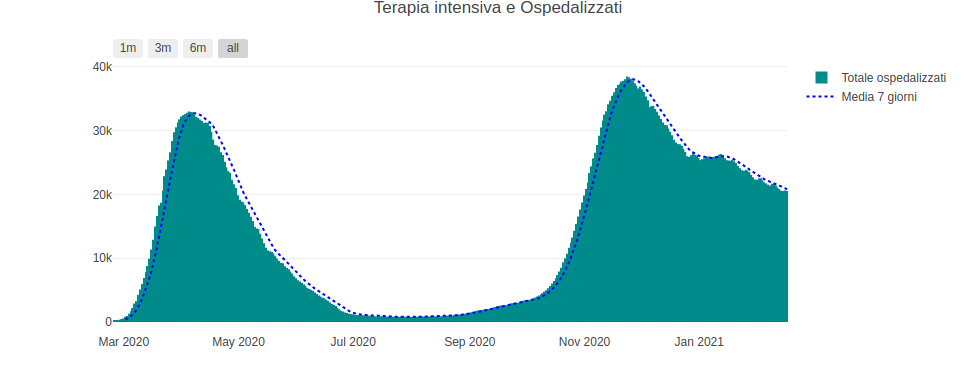
\includegraphics[width=14cm]{ospedalizzati}
    \caption{Terapia intensiva e ospedalizzati}
    \label{fig:ti_ospdedalizzati}
\end{figure}

% TODO: media 7gg: decessi giorn vs contagi giorn

% TODO: % casi positivi / casi testati

\subsection{Nuovi casi e decessi}
Nella figura \ref{fig:casi_decessi} viene mostrato l'andamento dei positivi e dei decessi.
In questo grafico è anche possibile selezionare l'intervallo temporale, agendo sulla barra in basso.
\begin{figure}[htp]
    \centering
    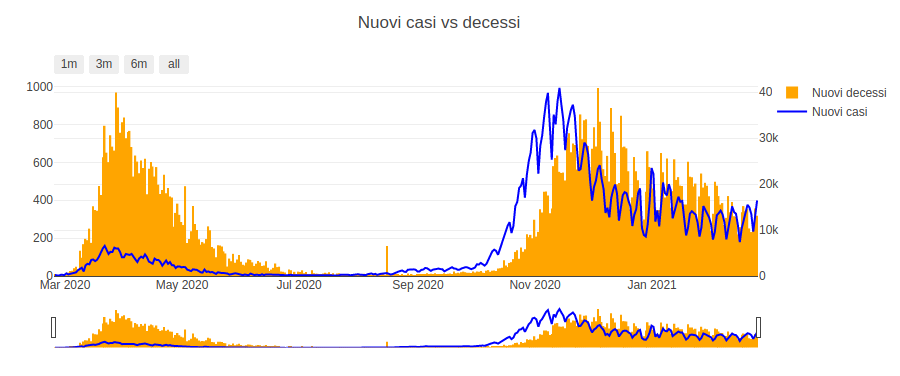
\includegraphics[width=14cm]{casi_decessi}
    \caption{Nuovi casi e nuovi decessi}
    \label{fig:casi_decessi}
\end{figure}

\section{Dashboard Lombardia}
\subsection{Andamento dei contagi}
Nella figura \ref{fig:andamento_lomb} è raffigurato l'andamento dei contagi nella regione Lombardia.
In giallo la linea della media mobile a 7 giorni.
\begin{figure}[htp]
    \centering
    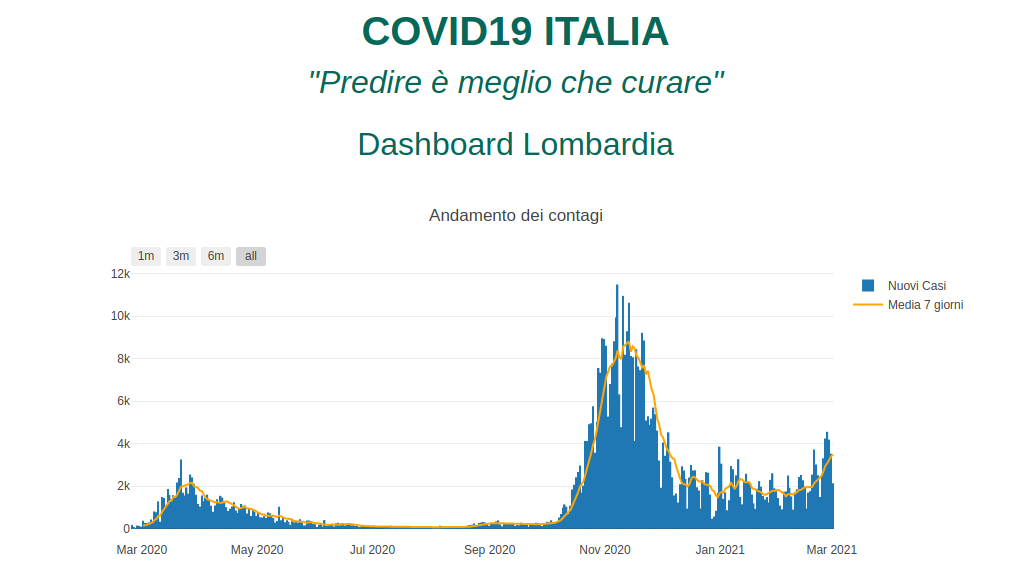
\includegraphics[width=12cm]{img/lomb/andamento_lomb.png}
    \caption{Andamento dei contagi in Lombardia}
    \label{fig:andamento_lomb}
\end{figure}

\subsection{Percentuale positivi sui casi testati}
Nella figura \ref{fig:positivi_testati_lomb} rappresenta la percentuale del rapporto tra i nuovi casi / totale dei casi e il numero dei casi testati tramite tamponi.
La linea gialla indica l'andamento dei \emph{nuovi casi testati}, mentre quella blu indica il \emph{totale dei casi testati}.
Le linee "punteggiate" indicano le medie mobili a 3 giorni.
\begin{figure}[htp]
    \centering
    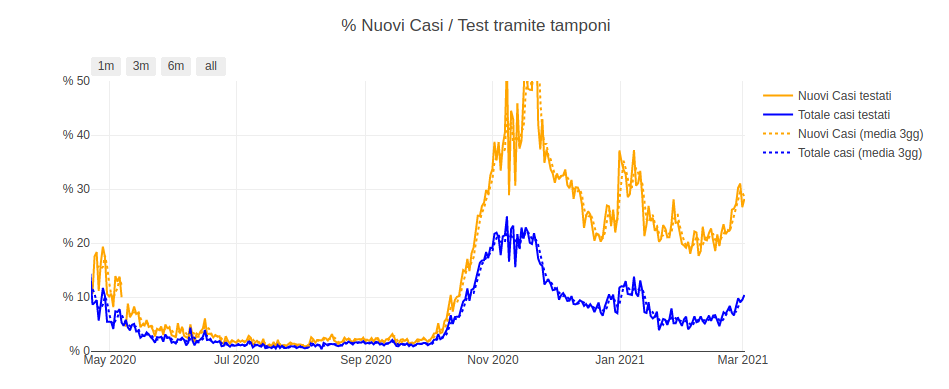
\includegraphics[width=12cm]{img/lomb/casi_tamp_lomb.png}
    \caption{Andamento dei contagi in Lombardia}
    \label{fig:positivi_testati_lomb}
\end{figure}

\subsection{Casi normalizzati}
Nella figura \ref{fig:casi_norm_lomb} è possibile osservare l'andamento dei casi normalizzati nella regione Lombardia.
\begin{figure}[htp]
    \centering
    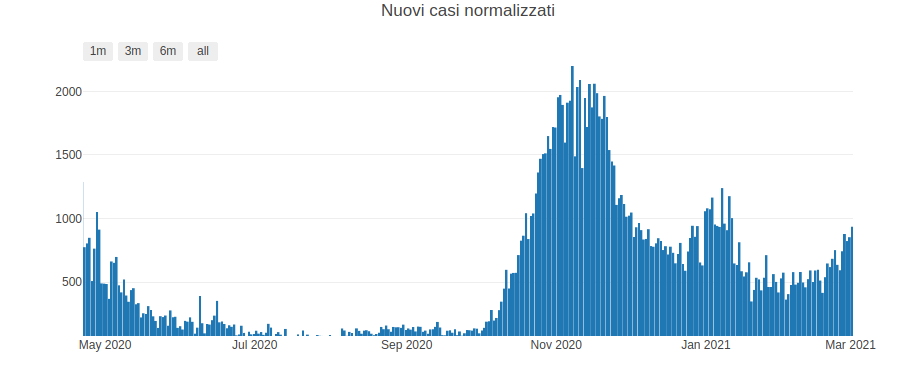
\includegraphics[width=14cm]{img/lomb/casi_norm_lomb.png}
    \caption{Andamento dei casi normalizzati}
    \label{fig:casi_norm_lomb}
\end{figure}

\subsection{Ospedalizzazioni}
Nella figura \ref{fig:ospedalizzati_lomb} si può osservare l'andamento delle ospedalizzazioni nella regione Lombardia.
In arancione è raffigurata la linea della media mobile a 7 giorni.
\begin{figure}[htp]
    \centering
    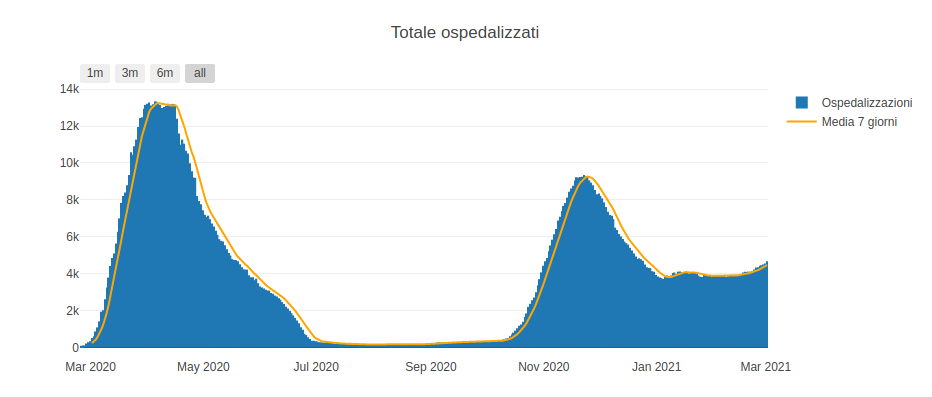
\includegraphics[width=14cm]{img/lomb/ospedalizzati_lomb.png}
    \caption{Andamento delle ospedalizzazioni in Lombardia}
    \label{fig:ospedalizzati_lomb}
\end{figure}

\subsection{Decessi giornalieri}
La figura \ref{fig:decessi_lomb} mostra l'andamento dei decessi nella regione Lombardia.
La linea blu indica la media mobile a 7 giorni.
\begin{figure}[htp]
    \centering
    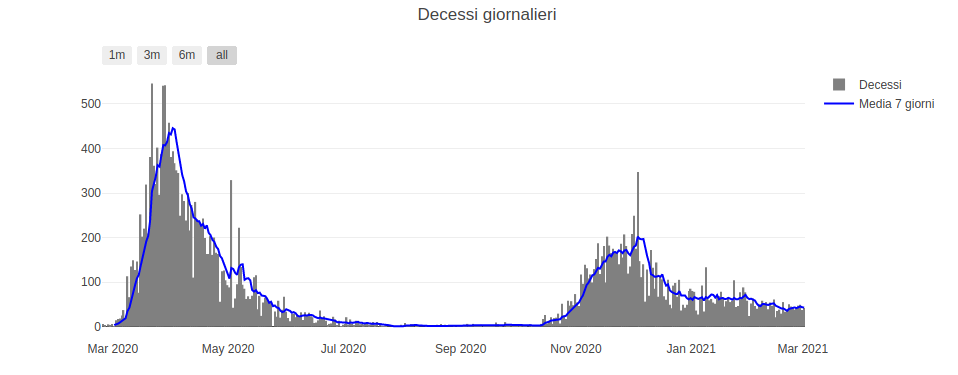
\includegraphics[width=14cm]{img/lomb/decessi_lomb.png}
    \caption{Andamento dei deceduti}
    \label{fig:decessi_lomb}
\end{figure}

\subsection{Terapia intensiva}
La figura \ref{fig:ti_lomb} mostra l'andamento dei pazienti ricoverati negli ospedali lombardi in terapia intensiva, dall'inizio della pandemia.
\begin{figure}[htp]
    \centering
    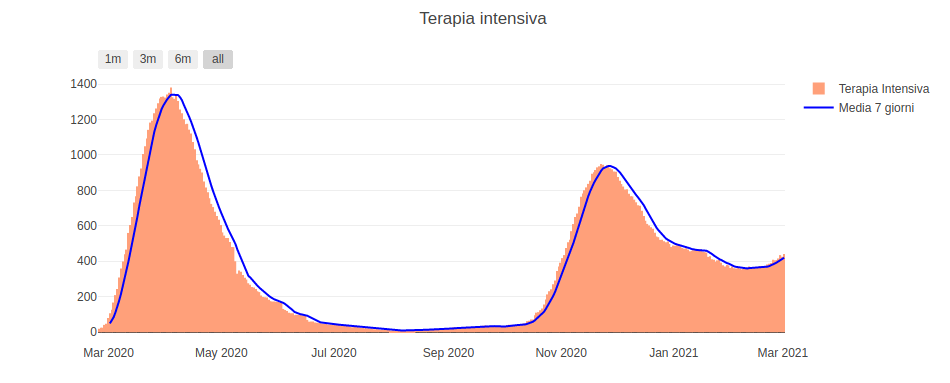
\includegraphics[width=12cm]{img/lomb/ti_lomb.png}
    \caption{Andamento della terapia intensiva}
    \label{fig:ti_lomb}
\end{figure}

\section{Dashboard Regioni}
Nella dashboard regioni, selezionando dal menù a tendina la regione di interesse (nella figura \ref{fig:tendina}), è possibile visualizzarne i dati.
I grafici contenuti all’interno della dashboard regioni sono analoghi ai precedenti, e riguardano
\begin{itemize}
\item Andamento dei contagi
\item Percentuale nuovi casi sui tamponi effettuati
\item Totale ospedalizzati
\item Decessi giornalieri
\item Terapia intensiva
\end{itemize}
\begin{figure}[htp]
    \centering
    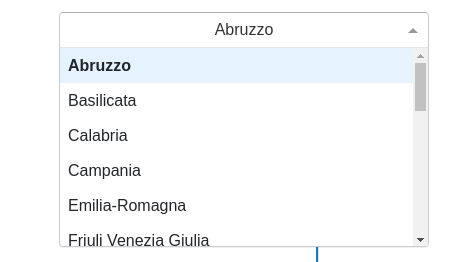
\includegraphics[width=10cm]{img/tendina_regioni.png}
    \caption{Selezione della regione}
    \label{fig:tendina}
\end{figure}

\begin{figure}[htp]
    \centering
    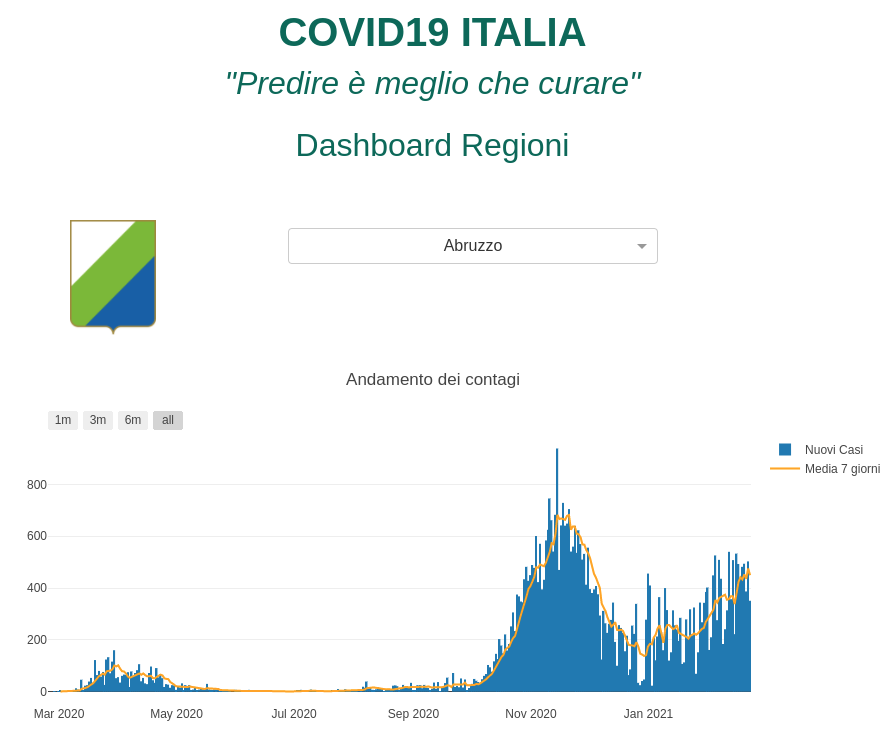
\includegraphics[width=12cm]{dash_regioni}
    \caption{Visualizzazione della regione Abruzzo}
    \label{fig:dash_regioni}
\end{figure}